% !TEX root = ../paper.tex
\section{Discussion}
Our results have shown that using semantic similarity can classify usefulness of comments and our approach also can reduce human effort ant error prone of manual classification. Besides the results, we also found interesting findings in our case study. We discuss these findings as follows:

% tuning the F score for precision and recall
%Depending on the use case, we can fine-tune the F-score to give more weight to recall or precision.
%For instance, if we wanted to measure the amount of useful comments within a large dataset, more weight can be given to precision, sacrificing some useful comments.
%If we wanted to modify a code review software such that it displays useful comments more prominently, more weight can be given to recall.

% examples.
\subsection{What kind of comments cannot be classified using semantic similarity?}
From the results of RQ1, we found that some comments were not determined by our models. Specifically, we were interested in comments with useful class (\texttt{YES} = 3) and useless class (\texttt{YES} = 0). To investigate the reason behind this, we observed these comments and the corresponding commit messages. We found that there were few common keywords between comments and commit messages and their length are relatively unequal. This makes low similarity values and low dissimilarity values as they shown in  bottom left white area in Fig. \ref{fig:scatter} which our models cannot determine.


%In some cases, similarity and dissimilarity failed to measure the usefulness of the comment,
%due to the same word being used in a different context.
%For example, consider this excerpt from the commit message: \emph{``In the no-assert case, make Q\_ASSERT decay to Q\_ASSUME. I can confirm
%better code generation with GCC at least.''}
%This comment, \emph{``I'll study the generated code a bit more,''} is just an author's response, and thus is not technically contributing. However, it is classified as a useful comment. This may be caused by the word \emph{generate} which appears in both documents.


%\subsection{Binary Classification}
\subsection{How much impact of unclear class on model construction?}
 % noisy data, and binary classification
Our training data contains much variability because there are disagreements between our judgment of ``usefulness,'' rendering our results unclear; they cannot be classified as either useful or not useful.
This impacts the trade-off between the precision and recall for our model, and consequently, the F$_1$ score.

Another approach we tried is to perform a \emph{binary classification}.
This means we assume that there are no unclear or undetermined comments; only useful and useless.
For this, we removed the samples with 1 and 2 \texttt{YES} votes from our data set. 209 samples without disagreements are left.
By performing cross-validation using only samples with 0 and 3 \texttt{YES} votes, we obtained a much better F$_1$ score of 0.896.

We could not objectively measure the F$_1$ score for all samples, because giving positive or negative classification to 1 and 2-scored samples introduces a bias.
However, the results seen in Fig.\ref{fig:binary} suggests that the binary classifier tends to gives positive classification to samples with score of 2 more than samples with score of 1, and the \emph{vice versa} for negative classification. 

\begin{figure}[h]
\centering
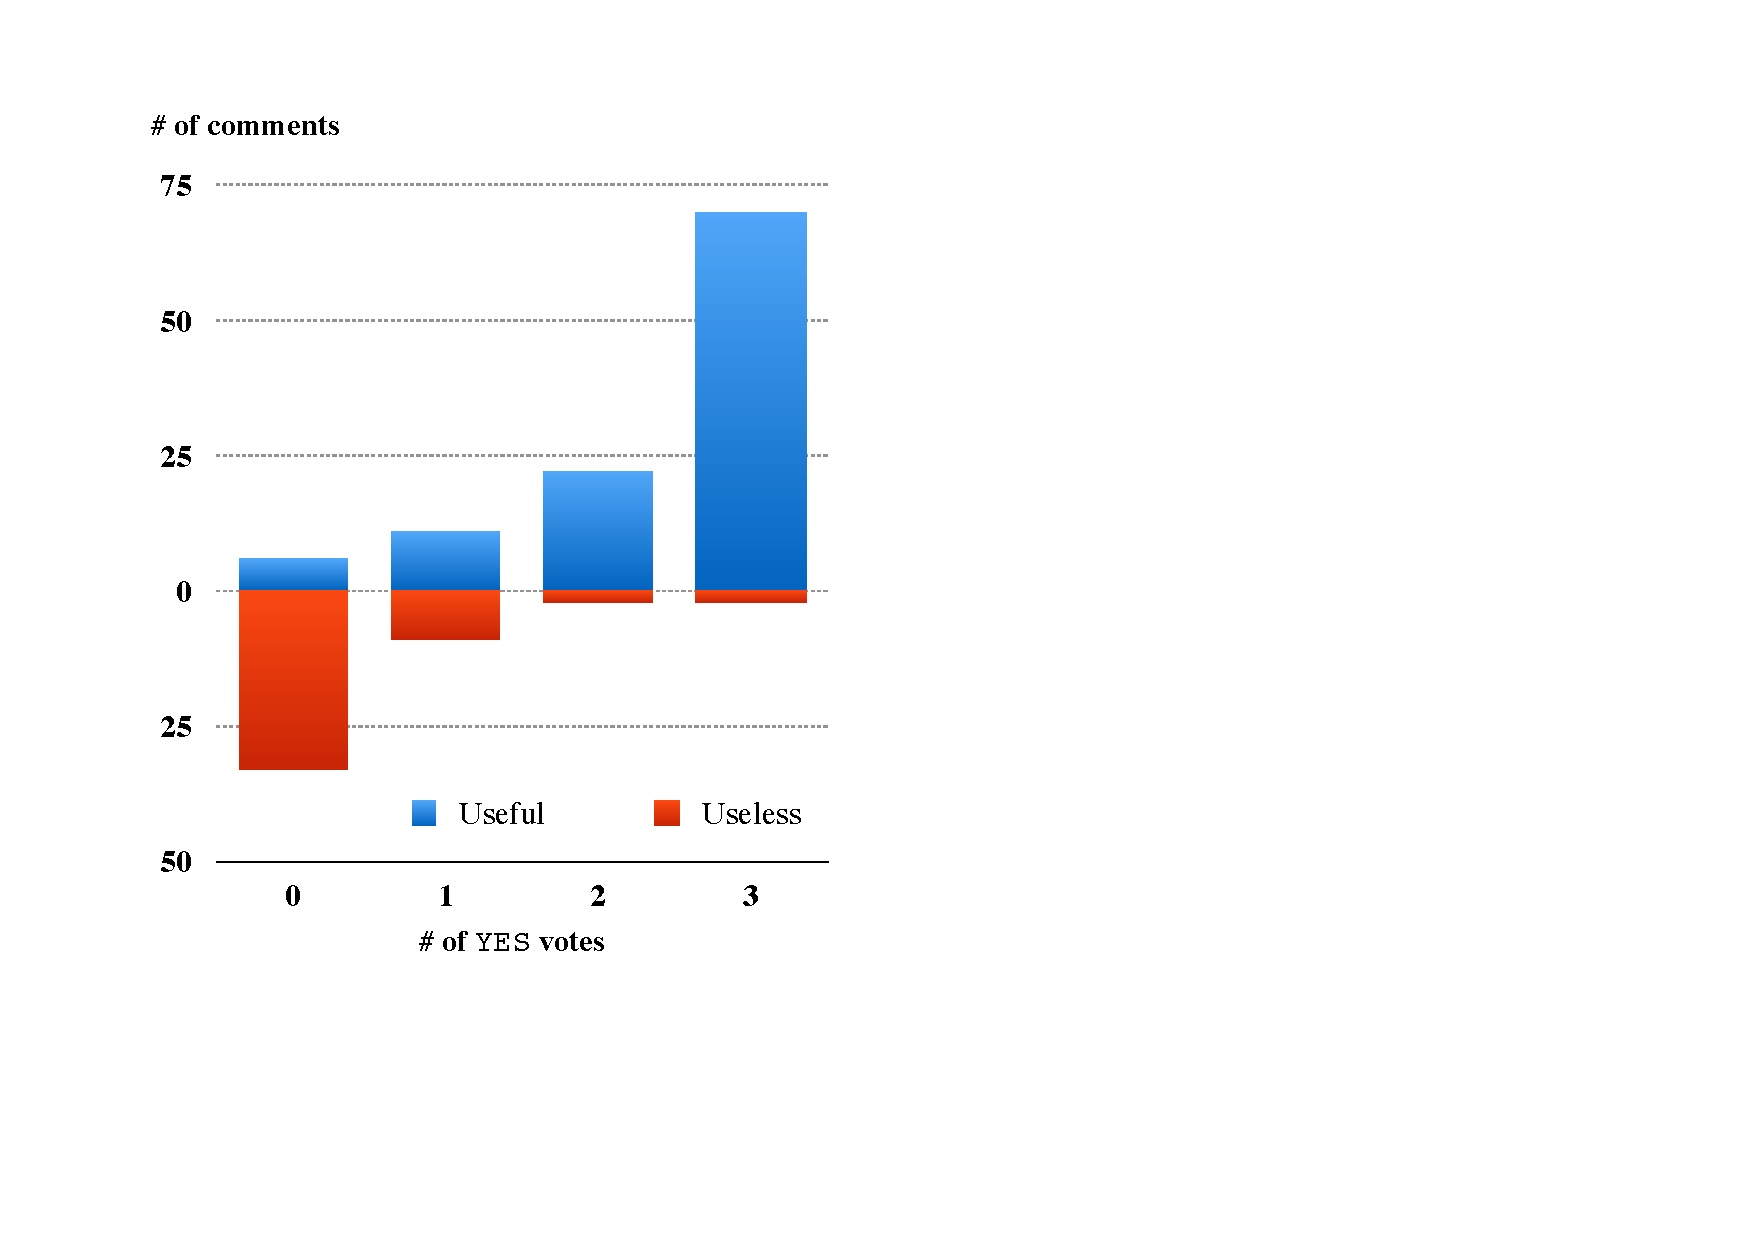
\includegraphics[width=2.5in]{posneg}
\caption{The amount of comments by score classified by the binary classifier.}
\label{fig:binary}
\end{figure}
\subsection*{Can other text mining techniques be used to classify discussions?}
To find relevance between comments and the corresponding commit message, topic modeling technique can be used as the study of \cite{Barua2012a}. This technique discovers topics for a given collection of documents. However, in MCR context, the documents generally is short descriptions and short discussions. 
The topic modeling technique would generate topics that include diverse actual topics of documents since the content of documents is insufficient to determine. We have applied Latent Dirichlet allocation (LDA), which is a well-known model of topic modeling techniques, on our data set. We found that the generated topics were diverse and some of them cannot did not have a relation between documents and their topics. Therefore, the topic modeling cannot be used to classify discussions. Others techniques will be investigated in our future work to improve our approach.

%\subsection{Reasons of Classification}
% reasons for classification as useful or not useful
\subsection*{What decisions are made during the manual classification?}
During manual comment usefulness assessment, we recorded the participants' rationale to verify that the comments are actually technically or little direct contribute to the proposed changes. We can summarize that most of reason for \texttt{YES} voting are: the comments 1) contain new information 2) contain constructive suggestions, 3) discuss directly to the proposed changes, and 4) discuss the technical matters. For \texttt{NO} voting, we can summarize that the comments 1) are chatting (just communication), 2) little direct to the proposed changes, 3) discuss about process workflow and supporting system i.e. Git and Gerrit.
%During the training process, reasons for the judgment are recorded. Examples of reasons for positive comments include:
%
%\begin{itemize}
%	\item they contain new information;
%	\item they contain constructive suggestions;
%	\item they discuss directly about the change; and
%	\item they discuss technical matters.
%\end{itemize}
%
%Examples of reasons for negative comments include:
%
%\begin{itemize}
%	\item chatting (i.e. no new information, just communication);
%	\item not discussing directly about the change;
%	\item discussing about the process workflow; and
%	\item discussing about Git or Gerrit itself.
%\end{itemize}

\subsection{Can the determined thresholds in this study be used to other projects?} 
In this study, we determined the similarity conditions using training set in Qt project and the results show that the conditions can classify usefulness of comments. However, to apply our approach on other projects, preparing training set is still required and it cost human effort. To fully automate this approach, we will investigate the use of similarity conditions for cross projects. Thus, additional studies are needed to improve our approach. 

